%Preamble
%%%%%%%%%%%%%%%%%%%%%%%%%%%%%%%%%%%%%%%%%%%%%%%%%%%%%%%%%%%%%
\documentclass[]{beamer}
\usetheme{Boadilla}

%%%%%%%%%%%%%%%%%%%%%%%%%%%%%%%%%%%%%%%%%%%%%%%%%%%%%%%%%%%%
%Packages
%%%%%%%%%%%%%%%%%%%%%%%%%%%%%%%%%%%%%%%%%%%%%%%%%%%%%%%%%%%%
\usepackage{amsmath}
\usepackage{booktabs} %nicer tables
\usepackage[utf8]{inputenc}

\usepackage{csquotes}
\usepackage{float}
\usepackage{graphicx}
\usepackage[justification=centering,singlelinecheck=off]{caption}
\usepackage[justification=centering, skip=3pt,font=small,margin=0pt]{subcaption}
\usepackage{tabularx}
\usepackage{adjustbox} %\resizebox and \adjustbox command
\usepackage{tikz}

%%%%%%%%%%%%%%%%%%%%%%%%%%%%%%%%%%%%%%%%%%%%%%%%%%%%%%%%%%%%
% Commands
%%%%%%%%%%%%%%%%%%%%%%%%%%%%%%%%%%%%%%%%%%%%%%%%%%%%%%%%%%%%
\let\Tiny=\tiny %workaround to get rid of some warnings

\newcommand{\sym}[1]{{#1}} % esttab outputs all asterisks inside \sym{}, which latex does not recognise by default

\newcommand{\backupbegin}{
	\newcounter{finalframe}
	\setcounter{finalframe}{\value{framenumber}}
}
\newcommand{\backupend}{
	\setcounter{framenumber}{\value{finalframe}}
}

%%%%%%%%%%%%%%%%%%%%%%%%%%%%%%%%%%%%%%%%%%%%%%%%%%%%%%%%%%%%
% Meta Info
%%%%%%%%%%%%%%%%%%%%%%%%%%%%%%%%%%%%%%%%%%%%%%%%%%%%%%%%%%%%
\title[Rolodex]{Rolodex}
\author[Marco \& Steven\& Herpfer]{Marco Ceccarelli  \inst{1},  Christoph Herpfer \inst{2} \and Steven Ongena \inst{1}}

\institute[]{
      \begin{tabular}{c c c}
        \inst{1} Swiss Finance Institute and UZH & \hspace*{0.01cm}  &    \inst{2} Emory University, Goizueta Business School  \\
      	\vspace*{0.5cm} 
\includegraphics[scale=0.13]{../../Writeup/figures/sfilogo.pdf}   & \hspace*{0.1cm}  &  
\includegraphics[scale=0.20]{../../Writeup/figures/GBS_hz_280} %\\
%      	
\includegraphics[scale=0.12]{../../Writeup/figures/sfilogo} & \hspace*{0.5cm} & 
      \end{tabular}             
    
     \vspace*{1em}
     \inst{1} Swiss Finance Institute and UZH \and %
     \inst{2} Emory University, Goizueta Business School
          }


%\date[December 13, 2017]{December 13, 2017}
\date[]{}
\setbeamertemplate{caption}[numbered]

\beamertemplatenavigationsymbolsempty %remove the navigation symbols in the bottom right corner

\setlength\itemsep{1em}
 
 %%%%%%%%%%%%%%%%%%%%%%%%%%%%%%%%%%%%%%%%%%%%%%%%%%%%%%%%%%%%
%  Main Part
 %%%%%%%%%%%%%%%%%%%%%%%%%%%%%%%%%%%%%%%%%%%%%%%%%%%%%%%%%%%%
 
  \begin{document}
  

  
  \begin{frame}
    \titlepage
  \end{frame}


\section{Introduction}

%%%%%%%%%%%%%%%%%%%%%%%%%%%%%%%%%%%%%%%%%%%%%%%%%%%%%%%%%%%%%
%SLIDE
%%%%%%%%%%%%%%%%%%%%%%%%%%%%%%%%%%%%%%%%%%%%%%%%%%%%%%%%%%%%% 

  \begin{frame}[t]
    \frametitle{Introduction}


\begin{minipage}{0.45\linewidth}
	\begin{itemize}
		\item Iqbal Kahn, switched from Credit Suisse to UBS
		\item Kahn alleges he was followed by private investigators hired by Credit Suisse after his departere. They were afraid he might take bankers with him that would poach clients.
			\onslide<2->{ \item Tidjane Thiam, CEO of Credit Suisse, stepped down shortly after the scandal emerged.}
	\end{itemize}
\end{minipage}%
\begin{minipage}{0.6\linewidth}
	\begin{figure}[H]
		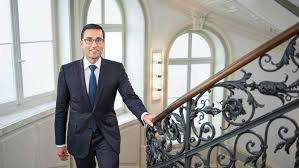
\includegraphics[scale=0.4]{../../Writeup/figures/Khan.jpg}
	\end{figure}
	\begin{figure}[H]
		\onslide<2->{ 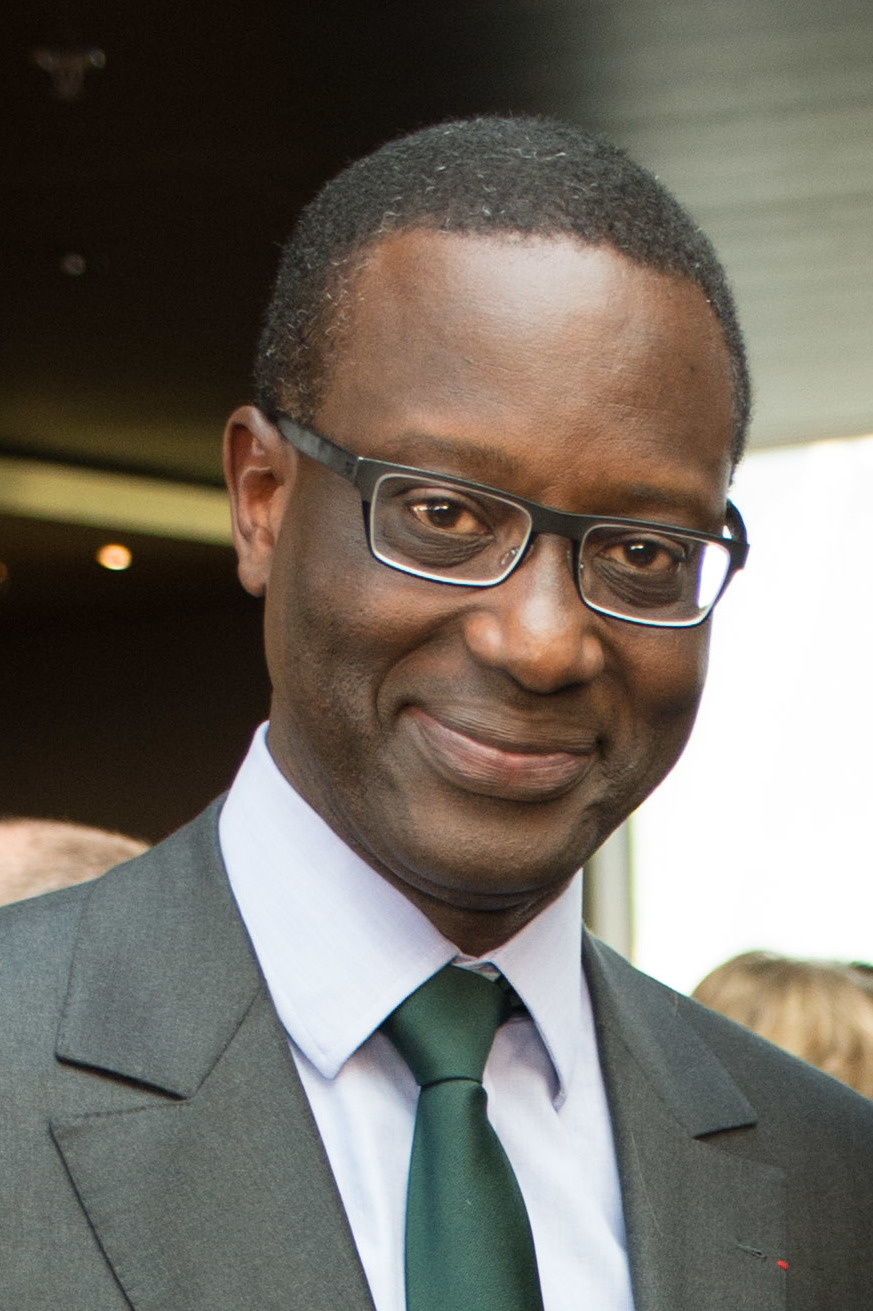
\includegraphics[scale=0.41]{../../Writeup/figures/Thiam.jpg}}
\end{figure}
\end{minipage}


%%%%%
%THIS! 
%https://www.reuters.com/article/us-jp-morgan-europe/jpmorgan-hires-commercial-bankers-leaders-across-europe-asia-idUSKCN1QG2SQ
%``JPMorgan Chase & Co on Wednesday named half a dozen people to a commercial banking team in Europe and new international and Asia-Pacific regional leaders, as the U.S. bank closes in on business clients it hopes to poach from rivals abroad. ''
%His team includes Claude Craciun in Paris, who joined from Societe Generale SA, Bernhard Brinker in Frankfurt, who joined from UniCredit Bank AG, Marco Mariano in Milan, who joined from HSBC, and Hein Broerse in Amsterdam, previously of Citigroup Inc. 
%%%%%

%suntrust merger:
%https://www.americanbanker.com/news/citizens-looks-to-poach-bb-t-suntrust-talent-but-should-expect-a-fight
%``The $161 billion-asset Citizens has already recruited one team of commercial bankers away from SunTrust, and its top commercial banker said Tuesday that he expects the merger — the industry’s largest in more than a decade — to lead to more banker defections.''
%McCree said Tuesday that Citizens has been adding around 300 new clients every year across its footprint, and it’s done so primarily by hiring local bankers in its newer markets. [...] “They are bringing clients with them, which is one of my goals when I hire people,” he said. McCree is Vice Chairman and Head of Commercial Banking at Citizens

%article on spying
%https://www.businessinsider.com/credit-suisse-ceo-tidjane-thiam-steps-down-after-spying-scandal-2020-2?r=US&IR=T

%article on another banker who took a single client call before starting job (investment banker)
%https://www.finews.com/news/english-news/34276-marco-illy-ubs-credit-suisse-investment-bank-switzerland-credit-suisse-notice-contract-dissolved-andrea-orcel-axel-lehmann-christine-novakovic

%sp global article poaching clients
%https://www.spglobal.com/marketintelligence/en/news-insights/research/ma-creates-poaching-opportunities-for-commercial-credits
%``Bankers often talk about C&I lending as a relationship-driven business, so an acquisition could force large clients to reconsider their lending partners. Commercial borrowers often select banks for reasons beyond the loan's terms and pricing, valuing institutions that can also deliver cash management, debt syndication or other services.''

%https://www.boyden.com/media/small-regional-banks-find-ease-poaching-large-bank-talent-588520/index.html
%The strategy gives smaller firms a crack at picking off large rivals' clients, says Jeff Davis, senior analyst at FTN Financial, a unit of First Horizon National Corp. (FHN). That's because business customers are notoriously loyal to their bankers.

%WSJ article on banks actively doing this:
%https://www.wsj.com/articles/SB10001424127887323530404578205842980922344
%Jim Schmitz, president of middle Tennessee for Regions, based in Birmingham, intends to add more Nashville bankers at the beginning of 2013. He said he would try to recruit from rival banks if he can find local lenders who can bring "relationships with companies we don't already have."

%CS hired private detective to follow Kahn out of fear he might poach bankers (not clients!)

  \end{frame}
 
%%%%%%%%%%%%%%%%%%%%%%%%%%%%%%%%%%%%%%%%%%%%%%%%%%%%%%%%%%%%%
%SLIDE
%%%%%%%%%%%%%%%%%%%%%%%%%%%%%%%%%%%%%%%%%%%%%%%%%%%%%%%%%%%%% 

\begin{frame}[t]
\frametitle{Banker poaching is not an isolated incident, and consistent with theory}

Banking is a relationship business and banks realize this broadly:


\onslide<1->{
	
	\textit{``Citizens has been adding around 300 new clients every year across its footprint, and it’s done so primarily by hiring local bankers in its newer markets. [...] They are bringing clients with them, which is one of my goals when I hire people”''}
	\linebreak
	\hspace*{2cm} -Don McCree, Head of Commercial Banking at Citizens}

\onslide<2->{
Theory:
    \begin{itemize}
	
	\item The ability of banks to create information about their borrowers is at the core of banking (e.g., Diamond, 1984; Petersen and Rajan, 1994; Berger and Udell, 1995). 
	\item The soft information of these relationships is concentrated in individual bankers (Liberti \& Petersen 2019). 


\end{itemize}


  %%%%%%%%%%%%%%%%%%%%%%%%%%%%%%%%%%%%%%%%%%%%%%%%%%%%%%%%%%%%%
  %SLIDE
  %%%%%%%%%%%%%%%%%%%%%%%%%%%%%%%%%%%%%%%%%%%%%%%%%%%%%%%%%%%%% 
  
  \begin{frame}[t]
  	\frametitle{Related literature and contribution}
  	       \framesubtitle{We contribute to the nascent literature on the role of bankers for large borrowers and the literature on information flows through capital providers}
  	\begin{itemize}

  		\item Frattaroli \& Herpfer (2020) bankers act as matchmakers between clients
  		\item Gao et al (2020) bankers face career consequences from making loans, Gao et al (2018) bankers can be distracted
		\item Herpfer (2017) shows that individual bankers in the U.S. syndicated loan market obtain significant information about their borrowers
		\item We have a unique advantage because we posses data on bankers working for separate banks and with multiple clients

		\item We show that
		\begin{itemize}
			\item Commercial bankers are a key link between banks and borrowers
			\item After a banker switches to a new employing bank, they bring over their prior clients
			\item These clients do not just come over once, but stay in the long term
			\item clients bring with them not just bank loans but the entire relationship, e.g. bond issuances
			\item Bankers that switch tend to have more, and more deep relationships with clients
%			\item
		\end{itemize}

  	\end{itemize}
  \end{frame}
  
  
 
  %%%%%%%%%%%%%%%%%%%%%%%%%%%%%%%%%%%%%%%%%%%%%%%%%%%%%%%%%%%%%
  %SLIDE
  %%%%%%%%%%%%%%%%%%%%%%%%%%%%%%%%%%%%%%%%%%%%%%%%%%%%%%%%%%%%% 
\section{Data}  
  
  \begin{frame}
    \frametitle{Data I}
       \framesubtitle{Bankers, Loans, Firms, Alliances}

We need data on loans, accounting variables, bankers, and other deals between . Data spans 2002 to 2013, sources are

    \begin{itemize}
    	\item LPC Dealscan
    	\item Compustat
    	\item CapitalIQ
    	\item Banker data from Herpfer (2017)
 
 	\end{itemize}
  \end{frame}

%%%%%%%%%%%%%%%%%%%%%%%%%%%%%%%%%%%%%%%%%%%%%%%%%%%%%%%%%%%%%
%SLIDE
%%%%%%%%%%%%%%%%%%%%%%%%%%%%%%%%%%%%%%%%%%%%%%%%%%%%%%%%%%%%% 


\begin{frame}[label=Data_I]
\frametitle{Data II: Individual Bankers}
\framesubtitle{Data on bankers from the signature pages of loan contracts} %\textcolor{red}{TBD: two steps: firs tonly talk loa contract and show picture loan contract, then exchange picture to signature page and talk name etc}


%Kramer: Linkedin: BA Harvard, MBA Berkley, BoA 1981 to 2004. Then non profit

\begin{minipage}{0.4\linewidth}
	\begin{itemize}
		\item Algorithm to identify publicly available loan contracts from EDGAR
		\onslide<2->{\item Extract the following data items from signature page:
			\begin{itemize}
				\item Bank Name
				\item Bank Role
				\item Person Name
				\item Person Title} 
		\end{itemize}
	\end{itemize}
\end{minipage}%
\begin{minipage}{0.6\linewidth}
	\begin{figure}[H]
		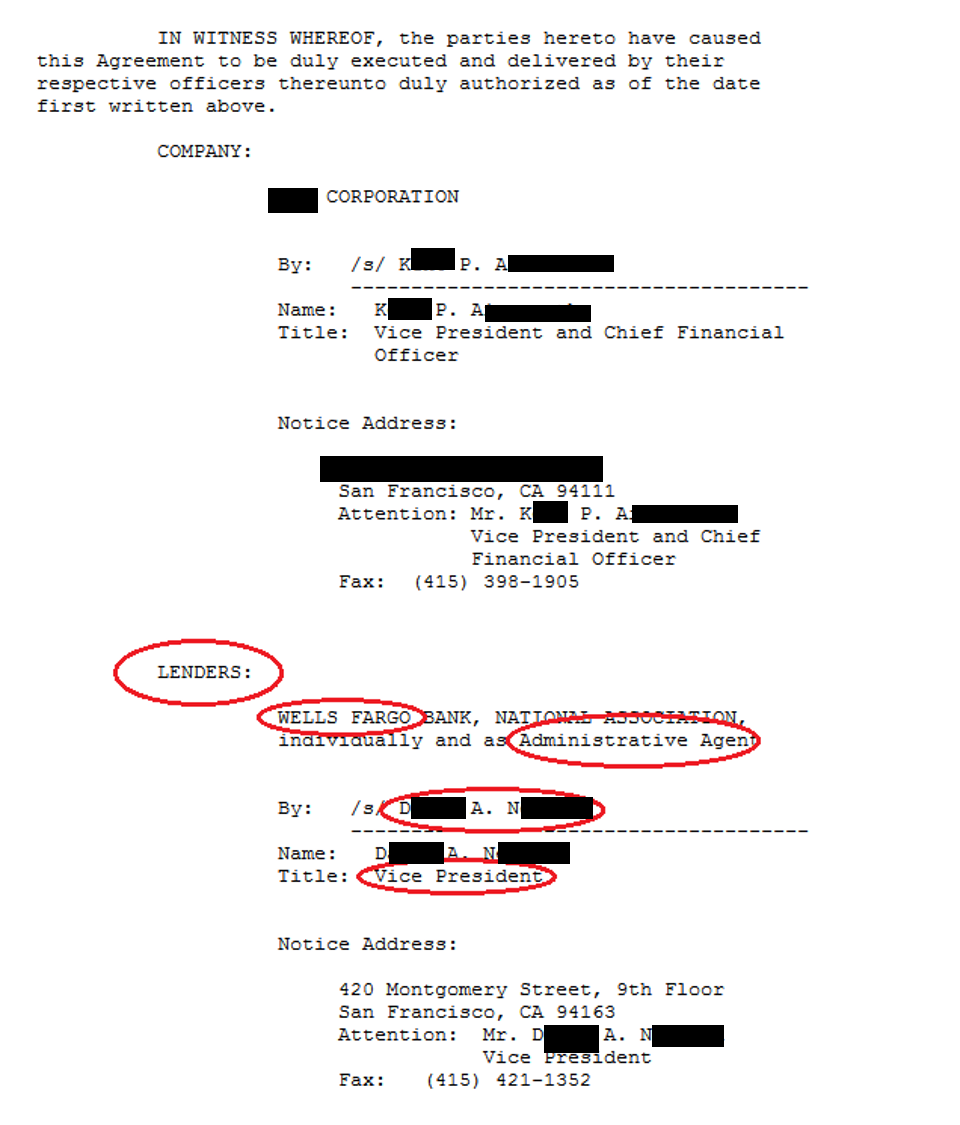
\includegraphics[scale=0.4]{../../Writeup/figures/signature_well_formated.png}
	\end{figure}
\end{minipage}

\begin{center}
	\vspace{-0.5em}
			\onslide<2->\hyperlink{Data_assurance}{\beamergotobutton{Quality assurance}}
\end{center}		

%%%%%%%%%%%%%%%%%%%%%%%%%%%%%%%%%%%%%%%%%%%%%%%%%%%%%%%%%%%%%
%SLIDE
%%%%%%%%%%%%%%%%%%%%%%%%%%%%%%%%%%%%%%%%%%%%%%%%%%%%%%%%%%%%% 


\end{frame}
      \begin{frame}
     \frametitle{Data III \textcolor{red}{TBD}}
     \framesubtitle{Banker overview}
     
     How many bankers, how many movers, how many banks
     
     \begin{itemize}
     	\item Number bankers
     	\item Movers
     	\item Average number deals during live
     	\item Average number clients 
     	
     \end{itemize}
 \end{frame}


   % 
   %%%%%%%%%%%%%%%%%%%%%%%%%%%%%%%%%%%%%%%%%%%%%%%%%%%%%%%%%%%%%
   %APPENDIX
   %%%%%%%%%%%%%%%%%%%%%%%%%%%%%%%%%%%%%%%%%%%%%%%%%%%%%%%%%%%%% 
   
   \appendix
   \backupbegin
   
   
   \begin{frame}[c]
   \centering
   \begin{huge}
   	\bigskip
   	Appendix
   \end{huge}
\end{frame} 
% 
% 

%%%%%%%%%%%%%%%%%%%%%%%%%%%%%%%%%%%%%%%%%%%%%%%%%%%%%%%%%%%%%
%SLIDE
%%%%%%%%%%%%%%%%%%%%%%%%%%%%%%%%%%%%%%%%%%%%%%%%%%%%%%%%%%%%% 

\begin{frame}[label=Data_assurance]
\frametitle{Data: Quality Assurance}
\framesubtitle{Most contracts feature signatures. Algorithm is reliable. Signatures proxy for involvement.}

Randomly sample 100 contracts to check quality of data:
\begin{itemize}
\item 65\% of contracts feature signatures, other contracts are dropped
\item 80\% of signatories are extracted successfully
\end{itemize}

Talk to various bankers in commercial lending
\begin{itemize}
\item Authorization of signature only for high ranking bankers
\item Bankers that sign are the ones negotiating
\item Titles are at the level of junior seniors
\item LinkedIn search: Relationship bankers, commercial bankers			
\end{itemize}

\begin{center}
\vspace{-0.5em}
\hyperlink{Data_I}{\beamergotobutton{Back to Data}}
\end{center}		


\end{frame}

\end{document}